\documentclass[../../main.tex]{subfiles}

\begin{document}

\section{Experimento 4: 45 períodos observados, 0 de dependencia} \label{sec:exp4}
En este experimento, seguimos tomando 45 períodos de observación pero con ninguno de
dependencia, por lo que consideramos que es el más extremo y en el que el desmpeño de las
redes y el PSM debería ser cercano.

Aquí, lo que diferencia a controles y tratados de los NiNi ya no es la presencia de una
determinada tendencia o no, sino que es el valor de la media de los efectos fijos,
que para los primeros es de 10 mientras que para los NiNi es de 7. Esto provoca que, al
graficar la variable para individuos de los diferentes grupos, no se observe ninguna
diferencia a simple vista, como se puede observar en la Figura \ref{fig:time_series_exp4}.
Sin embargo, al graficar el promedio por grupo de la variable en cada uno de los períodos
de tiempo, los promedios de tratados y controles se ubican siempre por encima de los de
los NiNi, como muestra la Figura \ref{fig:mean_time_series_exp4}.

\begin{figure}[ht]
    \centering
    \begin{minipage}{0.48\textwidth}
        \centering
        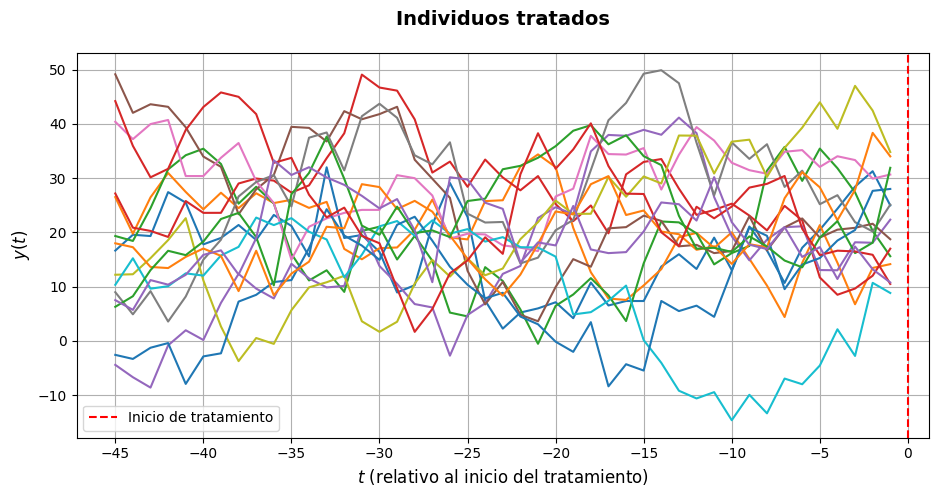
\includegraphics[scale=0.3]{figs/Exp4/tratados_sim13.png}
    \end{minipage}
    \hfill
    \begin{minipage}{0.48\textwidth}
        \centering
        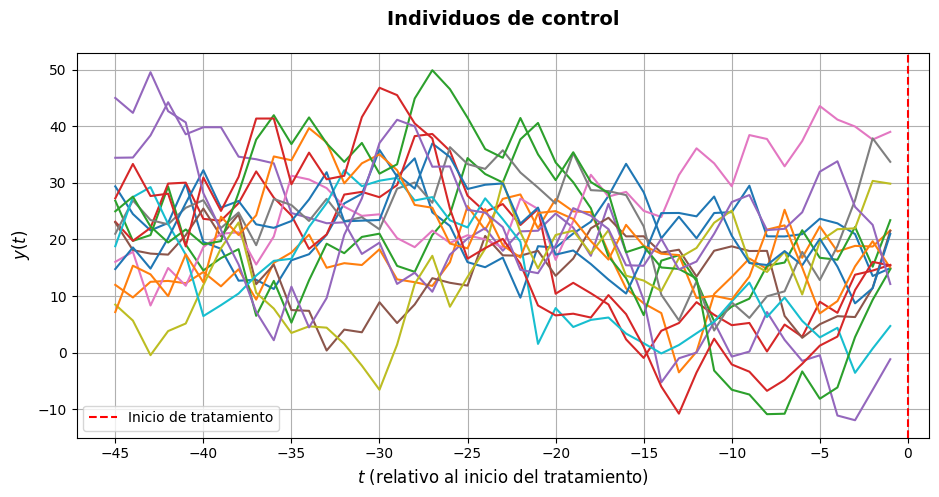
\includegraphics[scale=0.3]{figs/Exp4/controles_sim13.png}
    \end{minipage}
    \vspace{0.5em}
    \begin{minipage}{0.6\textwidth}
        \centering
        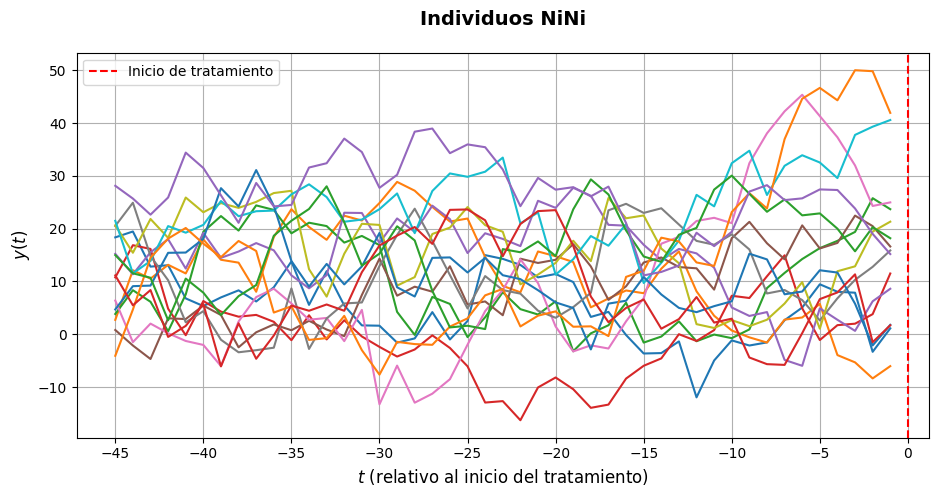
\includegraphics[scale=0.3]{figs/Exp4/ninis_sim13.png}
    \end{minipage}
    \caption{Ejemplos de series de tiempo generadas para cada grupo en el Experimento 4.
    La línea punteada roja indica el inicio de tratamiento para cada individuo. En este
    caso, no hay períodos de dependencia y no se observa ninguna tendencia ni en tratados
    ni en controles. A simple vista, no hay nada que diferencie a los individuos
    pertenecientes a estos dos grupos de los NiNi.}
    \label{fig:time_series_exp4}
\end{figure}

\begin{figure}[H]
    \centering
    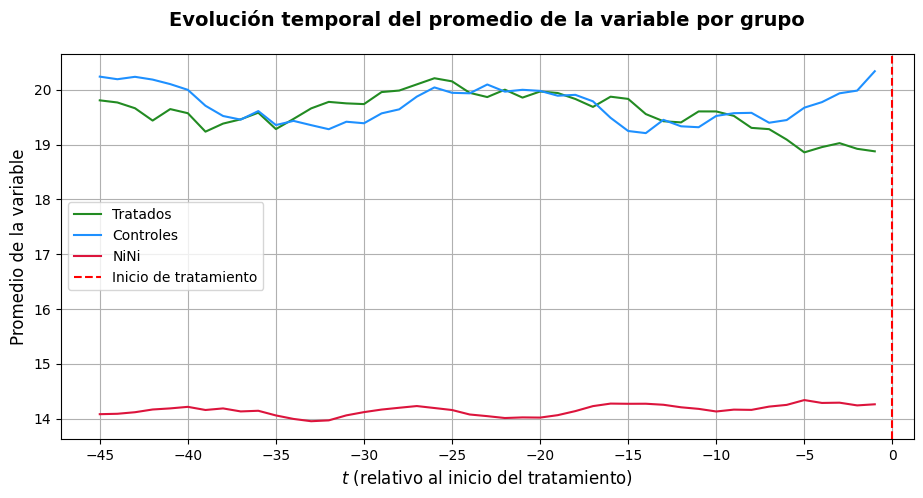
\includegraphics[scale=0.35]{figs/Exp4/promedios_sim13.png}
    \caption{Gráfico de la evolución temporal del promedio de la variable para los
    distintos grupos. El promedio se calcula por período con todos los individuos de cada
    grupo. Aquí se puede ver claramente que al disminuir el valor de la media de los
    efectos fijos en el grupo de los NiNi, los promedios por período están todos por
    debajo de los de los tratados y controles.}
    \label{fig:mean_time_series_exp4}
\end{figure}

Los resultados de este experimento se encuentran en la Tabla \ref{tab:results_exp4}, en
donde se observan valores bajos de todas las métricas en todos los modelos. Algo a notar
es que a comparación de los escenarios anteriores, la diferencia entre los resultados
obtenidos con las redes y con el PSM se redujo bastante, como habíamos planteado en
nuestras hipótesis. Más aún, si prestamos atención a la precisión, la obtenida con los
modelos es muy similar a la obtenida con el PSM.

De esta manera, los valores obtenidos indican que quitando los períodos de dependencia,
ninguno de los modelos es capaz de capturar una diferencia más ``implícita'' entre los
diferentes individudos, incluso con la mayor cantidad de períodos de observación
modelados.

\begin{table}[H]
    \centering
    \renewcommand{\arraystretch}{1.2}
    \begin{tabular}{|c|c|c|c|}
        \hline
         & \textbf{Puntaje} \(F_1\) & \textbf{Precisión} & \textbf{Cobertura} \\ \hline\hline
        \textbf{LSTM}
            & $0.28642 \pm 0.02401$ & $0.19572 \pm 0.02442$ & $\mathbf{0.55165 \pm 0.06813}$ \\ \hline
        \textbf{Convolucional}
            & $\mathbf{0.29402 \pm 0.01193}$ & $\mathbf{0.21026 \pm 0.00954}$ & $0.49111 \pm 0.03548$ \\ \hline
        \makecell{\textbf{LSTM +} \\ \textbf{Convolucional}}
            & $0.29149 \pm 0.01031$ & $0.20927 \pm 0.01094$ & $0.48416 \pm 0.03778$ \\ \hline
        \textbf{PSM}
            & $0.20161 \pm 0.01254$ & $0.20182 \pm 0.01252$ & $0.20140 \pm 0.01255$ \\
        \hline
    \end{tabular}
    \caption{Promedios y desviaciones estándar de las métricas \(F_1\), precisión y
    cobertura sobre la clase positiva (controles), evaluadas en el conjunto de test en las
    100 simulaciones del Experimento 4 con las diferentes arquitecturas de redes
    neuronales y el PSM.}
    \label{tab:results_exp4}
\end{table}

Los valores de los hiperparámetros seleccionados con mayor frecuencia como los óptimos se
encuentran en la Tabla \ref{tab:hyperparams_exp4}. La principal diferencia con respecto a
los escenarios anteriores es que aquí la tasa de aprendizaje de 0.0001 resultó como la más
elegida. Sin embargo, en este escenario no se obtuvieron buenos resultados, por lo que una
alternativa sería probar con un espacio de búsqueda más amplio, o incluso con otras
arquitecturas de redes neuronales.

\begin{table}[H]
    \centering
    \renewcommand{\arraystretch}{1.2}
    \begin{tabular}{|c|c|c|c|c|}
        \hline
            & \makecell{\textbf{Tamaño}\\\textbf{de lote}}
            & \makecell{\textbf{Neuronas en}\\\textbf{capas ocultas}}
            & \makecell{\textbf{Tasa de}\\\textbf{aprendizaje}}
            & \textbf{Dropout} \\ \hline\hline
        \textbf{LSTM}
            & 128 (37\%) & 128 (71\%) & 0.001 (99\%)  & 0.3 (55\%) \\ \hline
        \textbf{Convolucional}
            & 32 (43\%) & -           & 0.0001 (74\%) & 0.3 (97\%) \\ \hline
        \makecell{\textbf{LSTM +}\\\textbf{Convolucional}}
            & 32 (42\%) & 32 (39\%)   & 0.0001 (69\%) & 0.3 (99\%) \\
        \hline
    \end{tabular}
    \caption{Valores de hiperparámetros seleccionados con mayor frecuencia en las 100
    simulaciones en cada arquitectura en el Experimento 4. Cada celda contiene dicho valor
    y entre paréntesis el porcentaje de simulaciones en el que resultó ser el mejor, de
    acuerdo a la optimización realizada por Optuna mediante validación cruzada.}
    \label{tab:hyperparams_exp4}
\end{table}

\end{document}